\begin{figure}
  \centering
  \begin{subfigure}[t]{0.45\textwidth}
    \centering
    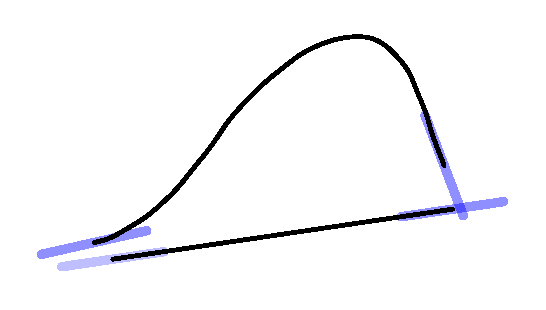
\includegraphics[width=0.6\linewidth]{img/latch-auto-endcaps.pdf}
    \caption{Automatic: latch where endcaps intersect.}
    \label{fig:latch-auto}
  \end{subfigure}
  \hspace{5mm}
  \begin{subfigure}[t]{0.45\textwidth}
    \centering
    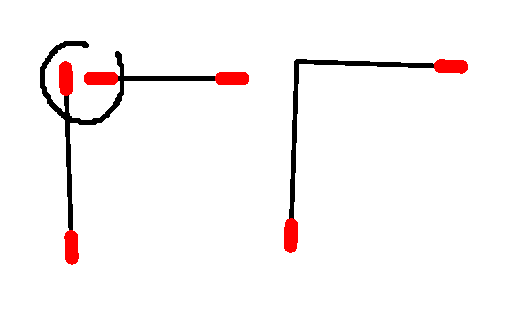
\includegraphics[width=0.6\linewidth]{img/latch-manual-endpoint.pdf}
    \caption{Endpoint latching.}
    \label{fig:latch-endpoint}
  \end{subfigure}

  \vspace{5mm}
  \begin{subfigure}[t]{0.45\textwidth}
    \centering
    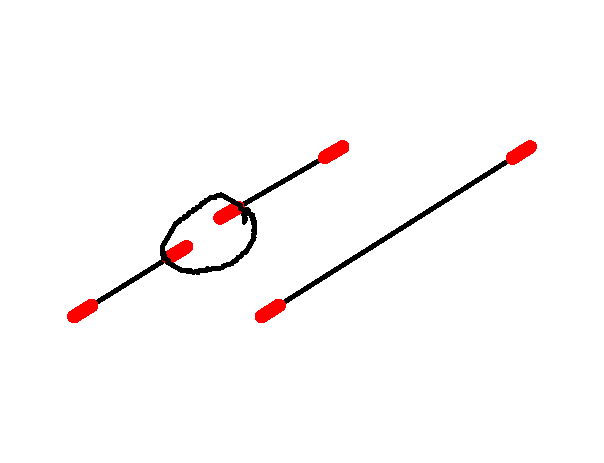
\includegraphics[width=0.6\linewidth]{img/latch-manual-continuation.pdf}
    \caption{Continuation latching.}
    \label{fig:latch-continuation}
  \end{subfigure}
  \begin{subfigure}[t]{0.45\textwidth}
    \centering
    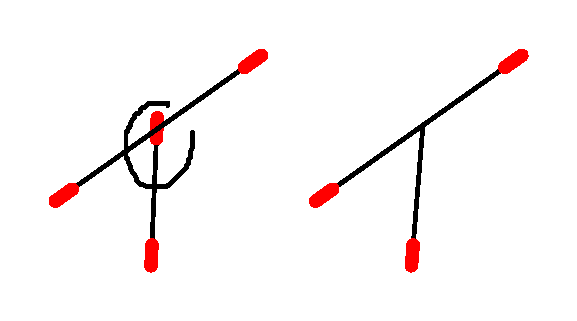
\includegraphics[width=0.6\linewidth]{img/latch-manual-tjunct.pdf}
    \caption{T-Junction latching.}
    \label{fig:latch-tjunct}
  \end{subfigure}
  \caption[Four kinds of latching]{Automatic and manual latching
    merges segments at a common point.}
  \label{fig:latch}
\end{figure}



